\documentclass[11pt]{book}
\usepackage[colorlinks = true,linkcolor = blue]{hyperref}
\usepackage[letterpaper]{geometry} % Custom margins
\usepackage{graphicx}
\usepackage[spanish]{babel}
\usepackage[T1]{fontenc}
\usepackage[utf8]{inputenc}
\usepackage{remreset}

\makeatletter
  \@removefromreset{section}{chapter}
\makeatother
\addto\captionsspanish{\renewcommand{\chaptername}{}}
\renewcommand{\thechapter}{Unidad \arabic{chapter}}
\renewcommand{\thesection}{S\arabic{section}}
\renewcommand{\thesubsection}{L\arabic{subsection}}
\setlength{\parindent}{0pt}

\begin{document}
\pagestyle{empty}
\newgeometry{letterpaper,left=15mm,top=50mm,bottom=0mm} % Custom margins
\begin{center}
  {\Huge Matem\'aticas 2}\\
  \vspace{2cm}
  \normalsize
  \textbf{\large Cuaderno de trabajo}\\
  para los alumnos de 2$^\circ$ de  Secundaria\\
  en el curso durante el ciclo escolar\\
  \textbf{2022-2023}\\
  \vspace{2.5cm}
  \small POR\\
  \Large J. C. Melchor Pinto\\[0.5em]
  \normalsize Profesor de asignatura en\\
  \vspace{1cm}
  
\includegraphics[width=4cm]{./Unidad 2/Images/LOGO_RDS_nobg}
\end{center}
\vspace{2cm}
%\include*{Functional/TitlePage}
\hspace{-16mm}
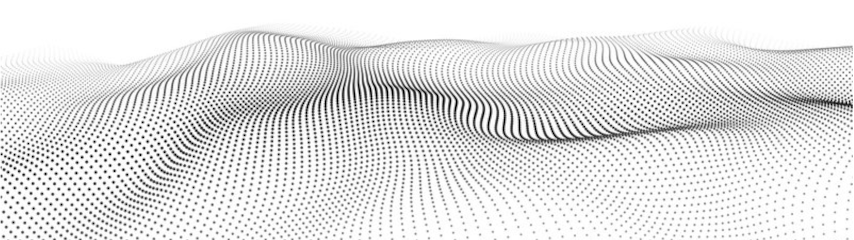
\includegraphics[width=\paperwidth]{./Unidad 2/Images/cover_bg}
\restoregeometry
\tableofcontents
\chapter{}

\section{Multiplicación de fracciones y decimales positivos.}
\subsection{Multiplicación de fracciones y decimales.}

\section{Multiplicación y división con fracciones y decimales positivos.}
\subsection{División con números fraccionarios.}
\subsection{Problemas de multiplicación y división de fracciones.}

\section{Multiplicación y división de números positivos y negativos.}
\subsection{Multiplicación de números positivos y negativos.}
\subsection{División de números positivos y negativos}
\subsection{Multiplicación y división de números con signo.}

\section{Potencia con exponente entero.}
\subsection{Productos de potencias enteras de la misma base.}
\subsection{Potencia de una potencia entera.}
\subsection{Cociente de potencias enteras de la misma base.}
\subsection{Potencias con exponente negativo y notación científica.}

\section{Raíces cuadradas.}
\subsection{Significado de la raíz cuadrada.}
\subsection{Aproximación de raíces cuadradas.}
\subsection{Cuadrados y raíces cuadradas.}

\section{Propiedades de polígonos.}
\subsection{Diagonales de un polígono.}
\subsection{Ángulos de un polígono.}

\section{Construcción de polígonos regulares.}
\subsection{Algunas construcciones de polígonos.}

\section{Conversión de unidades del SI y del sistema inglés.}
\subsection{Conversión entre unidades del SI.}
\subsection{Conversión entre unidades del sistema inglés.}
\subsection{Conversión de unidades del SI al sistema inglés y viceversa.}

\section{Histogramas, polígonos de frecuencias y gráficas de línea.}
\subsection{Histogramas}
\subsection{Polígonos de frecuencias}
\subsection{Gráficas de línea}
\subsection{Elección de la representación gráfica más adecuada.}

\chapter{}

\section{Proporcionalidad directa e inversa}
\subsection{Proporcionalidad directa e inversa}
\subsection{Problemas sobre proporcionalidad directa e inversa}

\section{Reparto Proporcional}
\subsection{Situaciones de reparto proporcional}

\section{Sistemas de ecuaciones lineales con dos inc\'ognitas}
\subsection{Ecuaciones lineales}
\subsection{Sistemas de ecuaciones lineales con dos inc\'ognitas}

\section{M\'etodos algebraicos de soluci\'on de sistemas de ecuaciones}
\subsection{Soluci\'on de sistemas de ecuaciones}
\subsection{Problemas sobre sistemas de ecuaciones lineales}

\section{Variabilidad lineal y proporcionalidad inversa}
\subsection{Situiaciones de variación lineal}
\subsection{Representaciones de proporcionalidad inversa}

\section{Modelos de variación lineal y proporcionalidad inversa}
\subsection{Modelos de variación lineal y proporcionalidad inversa}

\section{Per\'imetro y \'area de pol\'igonos regulares}
\subsection{Per\'imetro y \'area de pol\'igonos}

\section{\'Area del c\'irculo}
\subsection{Deducción de la f\'ormula del \'area del c\'irculo}


\section{Medidas de tendencia central, rango y desviación media}
\subsection{Medidas de tendencia central}
\subsection{Rango y dispersi\'on de datos}
\subsection{Desviaci\'on media}


%%% U3
\chapter{}

\section{Sucesiones y equivalencia de expresiones}
\subsection{Reglas aritméticas y equivalencias}

\section{Figuras geométricas y equivalencia de expresiones}
\subsection{Equivalencia de expresiones algebraicas}
\subsection{Expresiones de perímetros y áreas}

\section{Volumen de prismas rectos}
\subsection{Volumen de primas rectos con base en forma de polígono regular}
\subsection{Problemas de volumen de prismas rectos}

\section{Volumen de cilindros rectos}
\subsection{Volumen de cilindros rectos}
\subsection{Problemas de cilindros rectos}

\section{Desarrollos planos de prismas y cilindros rectos}
\subsection{Desarrollos planos}

\section{Probabilidad teórica}
\subsection{Definición de probabilidad teórica}
\subsection{Probabilidad teórica y frecuencial}

\end{document}






